\documentclass{article}

% if you need to pass options to natbib, use, e.g.:
%     \PassOptionsToPackage{numbers, compress}{natbib}
% before loading neurips_2026
\usepackage{graphicx}
\usepackage{subcaption}
\usepackage{placeins}
\usepackage{float}
% The authors should use one of these tracks.
% Before accepting by the NeurIPS conference, select one of the options below.
% 0. "default" for submission
\usepackage[preprint]{neurips_2026}
% the "default" option is equal to the "main" option, which is used for the Main Track with double-blind reviewing.
% 1. "main" option is used for the Main Track
%  \usepackage[main]{neurips_2026}
% 2. "position" option is used for the Position Paper Track
%  \usepackage[position]{neurips_2026}
% 3. "eandd" option is used for the Evaluations & Datasets Track
 % \usepackage[eandd]{neurips_2026}
 % if you want to opt-in for a de-anomymized submission (not recommended, but OK):
 %\usepackage[eandd, nonanonymous]{neurips_2026}
% 4. "creativeai" option is used for the Creative AI Track
%  \usepackage[creativeai]{neurips_2026}
% 5. "sglblindworkshop" option is used for the Workshop with single-blind reviewing
 % \usepackage[sglblindworkshop]{neurips_2026}
% 6. "dblblindworkshop" option is used for the Workshop with double-blind reviewing
%  \usepackage[dblblindworkshop]{neurips_2026}

% After being accepted, the authors should add "final" behind the track to compile a camera-ready version.
% 1. Main Track
 % \usepackage[main, final]{neurips_2026}
% 2. Position Paper Track
%  \usepackage[position, final]{neurips_2026}
% 3. Evaluations & Datasets Track
 % \usepackage[eandd, final]{neurips_2026}
% 4. Creative AI Track
%  \usepackage[creativeai, final]{neurips_2026}
% 5. Workshop with single-blind reviewing
%  \usepackage[sglblindworkshop, final]{neurips_2026}
% 6. Workshop with double-blind reviewing
%  \usepackage[dblblindworkshop, final]{neurips_2026}
% Note. For the workshop paper template, both \title{} and \workshoptitle{} are required, with the former indicating the paper title shown in the title and the latter indicating the workshop title displayed in the footnote.
% For workshops (5., 6.), the authors should add the name of the workshop, "\workshoptitle" command is used to set the workshop title.
% \workshoptitle{WORKSHOP TITLE}

% "preprint" option is used for arXiv or other preprint submissions
 % \usepackage[preprint]{neurips_2026}

% to avoid loading the natbib package, add option nonatbib:
%    \usepackage[nonatbib]{neurips_2026}

\usepackage[utf8]{inputenc} % allow utf-8 input
\usepackage[T1]{fontenc}    % use 8-bit T1 fonts
\usepackage{hyperref}       % hyperlinks
\usepackage{url}            % simple URL typesetting
\usepackage{booktabs}       % professional-quality tables
\usepackage{amsfonts}       % blackboard math symbols
\usepackage{nicefrac}       % compact symbols for 1/2, etc.
\usepackage{microtype}      % microtypography
\usepackage{xcolor}         % colors
\usepackage{amsmath}

% Note. For the workshop paper template, both \title{} and \workshoptitle{} are required, with the former indicating the paper title shown in the title and the latter indicating the workshop title displayed in the footnote. 
\title{Inferring Hidden Opponent Strategy Changes under Partial Observability in MOBA-like Environments}


% The \author macro works with any number of authors. There are two commands
% used to separate the names and addresses of multiple authors: \And and \AND.
%
% Using \And between authors leaves it to LaTeX to determine where to break the
% lines. Using \AND forces a line break at that point. So, if LaTeX puts 3 of 4
% authors names on the first line, and the last on the second line, try using
% \AND instead of \And before the third author name.


\author{
Po-Kai Huang \\
University of Minnesota \\
\texttt{huan3263@umn.edu}
\And
Erik Whittaker \\
University of Minnesota \\
\texttt{whitt369@umn.edu}
\And
Nicholas Pederson \\
University of Minnesota \\
\texttt{pede1116@umn.edu}
\AND
Adam Wagner \\
University of Minnesota \\
\texttt{Wagn1200@umn.edu}
\And
Nikita Tuli \\
University of Minnesota \\
\texttt{tuli0020@umn.edu }
}


\begin{document}


\maketitle


\begin{abstract}
  This project studies belief-based reasoning in partially observable environments with non-stationary opponents. Under such settings, the same observation sequence may be explained by multiple underlying strategies, making strategy inference fundamentally ambiguous. We propose a controlled MOBA-like environment in which opponent behavior is drawn from a predefined strategy library and may switch over time. The agent maintains a belief distribution over opponent strategies using Bayesian inference and uses this belief to support decision-making. To evaluate the role of belief-based reasoning, we compare belief-conditioned policies with observation-only baselines and introduce perturbed belief baselines to isolate the effect of correct inference. Our evaluation focuses on strategy inference accuracy, switch detection, and downstream decision performance. We further analyze under what conditions belief-based reasoning provides the greatest benefit. This work provides a controlled framework for understanding the role of reasoning in multi-agent environments with hidden and non-stationary dynamics.
\end{abstract}


\section{Introduction}

Partial observability and non-stationary opponents are two key challenges in multi-agent reinforcement learning \cite{hernandez2017survey, hernandez2019critique, papoudakis2019dealing}. In many multi-agent environments, agents must make decisions based on incomplete information about the environment while interacting with other agents whose behavior may change over time. These challenges are especially prominent in competitive settings, where the policies of other agents may evolve or switch strategies during interaction.

A large body of research has studied decision-making under partial observability (\cite{srinivasan2018acpo}) and learning in non-stationary multi-agent environments separately. However, in many real-world strategic scenarios, agents must address both challenges simultaneously. In such settings, an agent must reason about hidden opponent behaviors while also adapting to potential changes in those behaviors over time.

Some recent approaches have begun to consider this joint setting by combining opponent modeling with partially observable environments (\cite{zheng2018deep, wang2022bayesian, davies2020opponent}). In many of these methods, opponent behaviors are assumed to be drawn from a bounded or predefined library of strategies. While this assumption simplifies the learning problem, it still leaves a fundamental challenge unresolved.

Under partial observability and stochastic opponent policies, multiple latent strategies can produce indistinguishable observation sequences. This creates a fundamental ambiguity: apparent behavioral changes may reflect either stochastic variation or a true shift in the opponent’s underlying strategy.

This raises the central question of this work: does explicitly maintaining a belief over opponent strategies improve inference and decision-making under partial observability and non-stationarity?

Understanding this is important for designing agents that can robustly operate in real-world strategic environments, where both uncertainty and non-stationarity are unavoidable.

We make the following contributions:
\begin{itemize}
    \item We propose a controlled framework for studying belief-based reasoning under partial observability and non-stationary opponent dynamics.
    \item We implement a configurable Godot-based MOBA-like simulator with partial observability, scripted strategy switching, RL-compatible observation/action interfaces, and event logging for controlled evaluation.
    \item We isolate the effect of belief-based reasoning through a causal evaluation design, including perturbed belief baselines.
    \item We provide empirical analysis of when and under what conditions belief-based reasoning improves strategy inference, change detection, and downstream decision-making.
\end{itemize}

While prior work suggests that belief-based reasoning can improve decision-making under uncertainty, its practical impact on downstream performance remains unclear. In this work, we empirically evaluate whether belief inference improves policy learning in a partially observable, non-stationary environment.

Our results show that while belief models can infer opponent strategies and detect switching behavior, they do not necessarily improve task-level reward. Instead, belief signals provide modest improvements in behavioral stability and interpretability.


\section{Problem Statement}
We consider a partially observable multi-agent environment in which an agent interacts with an opponent whose underlying strategy is not directly observable and may change over time.

Let $\theta \in \Theta$ denote the opponent’s strategy, where $\Theta$ is a predefined strategy library. At each time step $t$, the agent receives an observation $o_t$ and observes the opponent’s action, but does not have access to $\theta_t$. The agent instead maintains a history of interactions $h_t = (o_1, a_1, \dots, o_t)$.

The goal of the agent is to infer the opponent’s current strategy from $h_t$ and use this information to support decision-making. However, under partial observability and stochastic policies, multiple strategies may induce similar observation sequences. This makes the mapping from $h_t$ to $\theta_t$ inherently ambiguous.

To address this, we consider maintaining a belief distribution over opponent strategies:
\[
b_t = P(\theta \mid h_t)
\]

which summarizes the agent’s inference over possible strategies given interaction history.

We study whether conditioning on this belief improves:
\begin{itemize}
    \item strategy inference accuracy,
    \item detection of strategy changes,
    \item and downstream decision-making performance.
\end{itemize}

In addition, we explicitly evaluate whether the inferred belief improves downstream decision-making performance when integrated into a reinforcement learning policy.

\section{Hypothesis}

We hypothesize that explicitly modeling a belief over opponent strategies improves inference and decision-making in partially observable environments with non-stationary opponents.

\textbf{H1 (Disambiguation):} Belief-based methods achieve higher strategy inference accuracy than observation-only methods, particularly when multiple strategies induce similar observation sequences.

\textbf{H2 (Change Detection):} Belief-based agents detect opponent strategy switches with lower delay and greater stability than observation-based agents.

\textbf{H3 (Environment Dependence):} The benefit of belief modeling is most significant in environments with both partial observability and strategy switching, and diminishes when the opponent strategy is stationary.

\section{Environment}

We design a simplified MOBA-like environment implemented in Godot for controlled study of hidden and non-stationary opponent behavior. The experimental setting used in this paper is a 1v1 lane-focused scenario: one learning-controlled agent interacts with one scripted opponent in a symmetric 2D arena with bushes, lane geometry, and optional lane objectives.

The simulator uses a continuous 2D space rather than a grid world. Partial observability is created through a limited vision radius, obstacle-aware line of sight, and bush regions that hide units unless they share the same bush or regain direct visibility.

At each time step, the learning agent receives a structured observation $o_t$ containing self state, visible agents, visible objects, and selected opponent-action information when the opponent is observed. In the current implementation, objects include lane minions, towers, and neutral monsters when enabled. The environment also exports per-step event counts such as takedowns and deaths for evaluation.

Agents act through a discrete 13-action interface consisting of 8 movement directions, hold, attack-hero, attack-nearest-minion, attack-tower, and retreat. The environment evolves according to these actions together with the scripted opponent policy.

Opponent behavior is governed by a latent strategy $\theta \in \Theta$, where each strategy corresponds to a stochastic policy. During an episode, the opponent may switch strategies at unknown time steps, inducing non-stationarity.

An episode terminates when a terminal condition is reached (e.g., objective completion or time limit).

\paragraph{Simulator Implementation.} The Godot side is responsible for world dynamics, combat resolution, visibility, scripted minion and tower interactions, structured observation export, and termination/reward signaling. Python is responsible for policy learning, belief updates, experiment control, and evaluation. This separation allows us to keep the environment mechanics fixed while varying the learning and inference methods on top of the same simulator.

\begin{figure}[H]
\centering
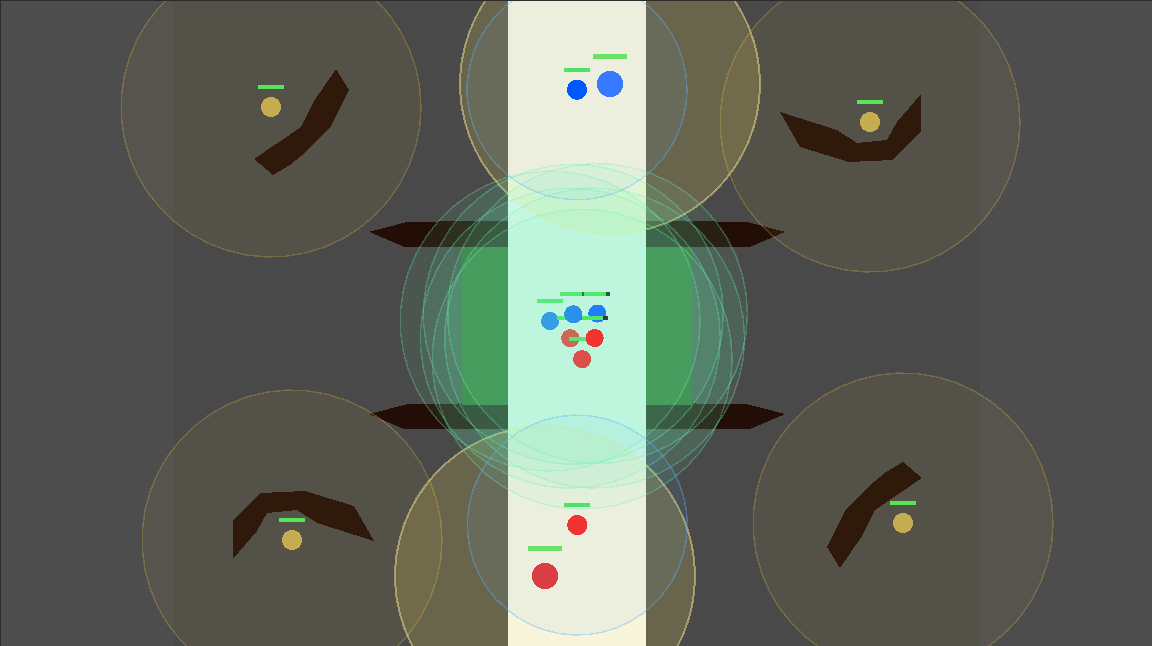
\includegraphics[width=0.82\linewidth]{images/example_sim.png}
\caption{Example state from the Godot-based simulator. The environment includes a central lane, bushes for partial observability, lane towers, lane minions, and neutral monsters, providing a controlled MOBA-like setting for opponent-modeling experiments.}
\label{fig:simulator_overview}
\end{figure}

\paragraph{Godot-Python Communication.} We used code from the open source package "Godot RL Agents" from \cite{beeching2021godotrlagents} to help facilitate communication between the Godot simulator and the Python RL scripts.  Godot RL Agents uses a socket-based interface. The simulator sends structured observations and event logs to the Python side at each time step, while the Python side sends back action commands. The Python side configures each experiment by sending a config message. This config message is a structured dictionary that the Godot side uses to determine what map to use, how many agents to include, and whether or not towers, minions, and neutral camps should be enabled. This allows for flexible experiment control and integration with standard RL algorithms.

The package includes a Godot plugin, which improves the ease of development with the Godot editor.  The plugin includes a sync node that handles communication. It can be set to "human," "training," or "Onnx Inference" mode. In "human" mode, the plugin allows for human playtesting by forwarding keyboard inputs as actions. In "training" mode, it waits for action commands from the Python side. In "Onnx Inference" mode, it runs a pre-trained ONNX model directly within Godot for inference without Python communication.

\section{Approach}

Our framework consists of two main components: opponent modeling via belief inference, and belief-conditioned policy learning.

\subsection{Opponent Strategy Model}

We assume that opponent behavior is governed by a latent strategy $\theta \in \Theta$, where each strategy corresponds to a distinct behavioral pattern (e.g., aggressive, neutral, or farming).

Each strategy defines a stochastic policy over actions:
\[
\pi_\theta(a \mid o) = \frac{\exp(\beta \cdot \text{score}_\theta(o,a))}{\sum_{a'} \exp(\beta \cdot \text{score}_\theta(o,a'))}
\]

where $o$ denotes the observation, $a$ denotes an action, $\beta$ controls the stochasticity, and $\text{score}_\theta(o,a)$ is a strategy-specific preference function.

In practice, the score function is implemented using heuristic features derived from the observation, such as relative position, target proximity, and combat context. These features encode prior assumptions about how different strategies behave in the environment.

\subsection{Belief Update}

The agent maintains a belief distribution over strategies:
\[
b_t(\theta) = P(\theta \mid h_t)
\]
where $h_t$ denotes the interaction history up to time $t$.

We update the belief using Bayesian inference:
\[
P(\theta \mid h_t) = \frac{P(h_t \mid \theta) P(\theta)}{\sum_{\theta'} P(h_t \mid \theta') P(\theta')}
\]

The likelihood is approximated as:
\[
P(h_t \mid \theta) \approx \prod_{k=1}^{t} \pi_\theta(a_k \mid o_k)
\]
assuming conditional independence of actions given $\theta$.

To improve computational stability, we perform updates in log-space and normalize the belief at each timestep. In addition, we use a smoothing factor to prevent the belief from collapsing too quickly to a single strategy.

\subsection{Policy Learning}

We train a policy conditioned on both observation and belief:
\[
\pi(a_t \mid o_t, b_t)
\]

The belief vector $b_t$ is concatenated with the observation $o_t$ and used as input to the policy network.

We optimize the policy using Proximal Policy Optimization (PPO) to maximize expected return:
\[
J(\pi) = \mathbb{E}\left[\sum_{t=0}^{T} \gamma^t r_t\right]
\]

We compare two policies:
\begin{itemize}
    \item Observation-only policy $\pi(a_t \mid o_t)$
    \item Belief-conditioned policy $\pi(a_t \mid o_t, b_t)$
\end{itemize}

Importantly, the policy is not designed to perform opponent reasoning implicitly. Instead, it serves as a controlled setting to evaluate whether explicitly provided belief representations improve downstream decision-making.

\subsection{Implementation Details}

The policy is implemented as a two-head actor-critic multilayer perceptron using separate networks for the actor and critic. 
Each network consists of two hidden layers with 64 units and \texttt{tanh} activations. 
The actor outputs logits for a categorical distribution over 13 discrete actions, while the critic outputs a scalar value estimate.

For the observation-only baseline, the input is the environment observation vector. 
For the belief-conditioned policy, a belief vector over opponent strategies is concatenated with the observation, resulting in an increased input dimension.

On the simulator side, the observation exported from Godot is a structured dictionary containing self state, visible agents, visible objects, and an extension field for observed enemy actions. This allows the belief module to access opponent behavior signals without directly exposing the hidden opponent strategy label. The simulator additionally records combat events such as deaths, enemy-agent takedowns, and enemy-minion takedowns, which are used both for reward shaping and for downstream evaluation.

We train the policy using PPO with a learning rate of $3\times 10^{-4}$, discount factor $\gamma=0.99$, and GAE parameter $\lambda=0.95$. 
The PPO clipping parameter is set to 0.2, with value loss coefficient 0.5 and entropy coefficient 0.003. 
Gradients are clipped with a maximum norm of 0.5. 
Each update is performed over 4 epochs with 4 minibatches, using batches of 1024 environment steps.

Training is conducted for a total of 102,400 timesteps with a maximum episode length of 1000 steps. 
We use a single learning agent in a 1v1 setting with partial observability and a vision range of 5.0.

For expert-guided training, expert actions are injected with an initial probability of 0.9, which decays linearly to 0 over 80 updates. 
The expert policy follows an aggressive strategy, while the opponent uses a neutral strategy during baseline training.

For experiments involving non-stationarity, opponent strategies switch during the episode according to a time-based schedule, 
with switch points sampled uniformly between steps 150 and 850.

\section{Evaluation}

The proposed framework is evaluated along three dimensions: strategy inference, strategy switch detection, and downstream decision performance.

\subsection{Strategy Inference}

Let $\theta_t$ denote the ground-truth opponent strategy at time $t$, and let $b_t(\theta)$ denote the inferred belief distribution. The predicted strategy is defined as:
\[
\hat{\theta}_t = \arg\max_{\theta} b_t(\theta)
\]

Inference accuracy is measured as:
\[
\text{Accuracy} = \frac{1}{T} \sum_{t=1}^{T} \mathbb{I}[\hat{\theta}_t = \theta_t]
\]

Under higher levels of observation ambiguity, belief-based methods are expected to maintain significantly higher classification accuracy, whereas observation-only baselines are expected to degrade due to indistinguishable behavior patterns.

\subsection{Strategy Switch Detection}

Let $t_{\text{switch}}$ denote the time step at which the opponent changes its strategy. The detection delay is defined as:
\[
\Delta = \min \{ t > t_{\text{switch}} : \arg\max_{\theta} b_t(\theta) = \theta_t \} - t_{\text{switch}}
\]

Belief stability is evaluated during non-switching intervals by measuring fluctuations in $b_t$ when $\theta_t$ remains constant.

We expect belief-based agents to detect strategy switches with lower delay and exhibit smoother belief transitions, whereas baseline methods may either respond more slowly or exhibit unstable fluctuations.

\subsection{Decision Performance}

Two policies are compared:
\begin{itemize}
    \item Observation-only policy $\pi(a_t \mid o_t)$
    \item Belief-conditioned policy $\pi(a_t \mid o_t, b_t)$
\end{itemize}

Performance is evaluated using the following metrics:
\begin{itemize}
    \item cumulative reward
    \item win rate
\end{itemize}

To isolate the effect of belief correctness, additional baselines with perturbed beliefs are introduced:
\begin{itemize}
    \item Random belief
    \item Shuffled belief
    \item Lagged belief
\end{itemize}

We expect belief-conditioned policies to achieve higher cumulative reward and win rate, particularly in non-stationary environments. In contrast, when the opponent's strategy is stationary, the performance gap between the two policies is expected to diminish.

These three evaluation dimensions allow us to separately assess (1) belief correctness and (2) its impact on downstream policy performance.

\section{Results}

\subsection{Training Dynamics}

We first analyze the training dynamics of PPO in the MOBA-like environment.

Figure~\ref{fig:ppo_action} shows the evolution of action group distributions over training. 
Initially, the agent exhibits movement-dominated behavior, while attack actions are relatively infrequent. 
As training progresses, the agent gradually increases its attack frequency and reduces unnecessary movement, 
indicating that it learns to engage more effectively with the environment.

This behavioral shift is further supported by combat statistics in Figure~\ref{fig:ppo_combat}. 
The number of enemy minion takedowns increases significantly over training, 
while interactions with enemy agents remain sparse. 
This suggests that the agent learns basic lane-clearing behavior but does not consistently engage in higher-risk combat.

Reward-related metrics in Figure~\ref{fig:ppo_reward} show partial improvement but remain highly unstable. 
While the cumulative reward improves compared to early training stages, 
it exhibits high variance and remains predominantly negative. 
Advantage estimates also show large fluctuations, indicating noisy and inconsistent learning signals.

Despite this, optimization metrics in Figure~\ref{fig:ppo_training} indicate stable training behavior. 
Both the PPO loss and value estimates decrease over time, 
and policy entropy gradually declines, suggesting that the policy is converging and exploration is being reduced.

However, these results highlight a key limitation: 
although PPO is able to learn structured behavior and achieve stable optimization, 
it fails to produce strong task-level performance in this environment.

To address this issue, we introduce expert-guided PPO, where expert actions are mixed into training with a decaying probability. 
As shown in later sections, expert guidance significantly improves learning stability and downstream performance. 
This suggests that exploration and credit assignment are major challenges in this environment, 
and that pure PPO is insufficient without additional guidance.

\begin{figure}[htbp]
    \centering

    \begin{subfigure}{0.48\linewidth}
        \centering
        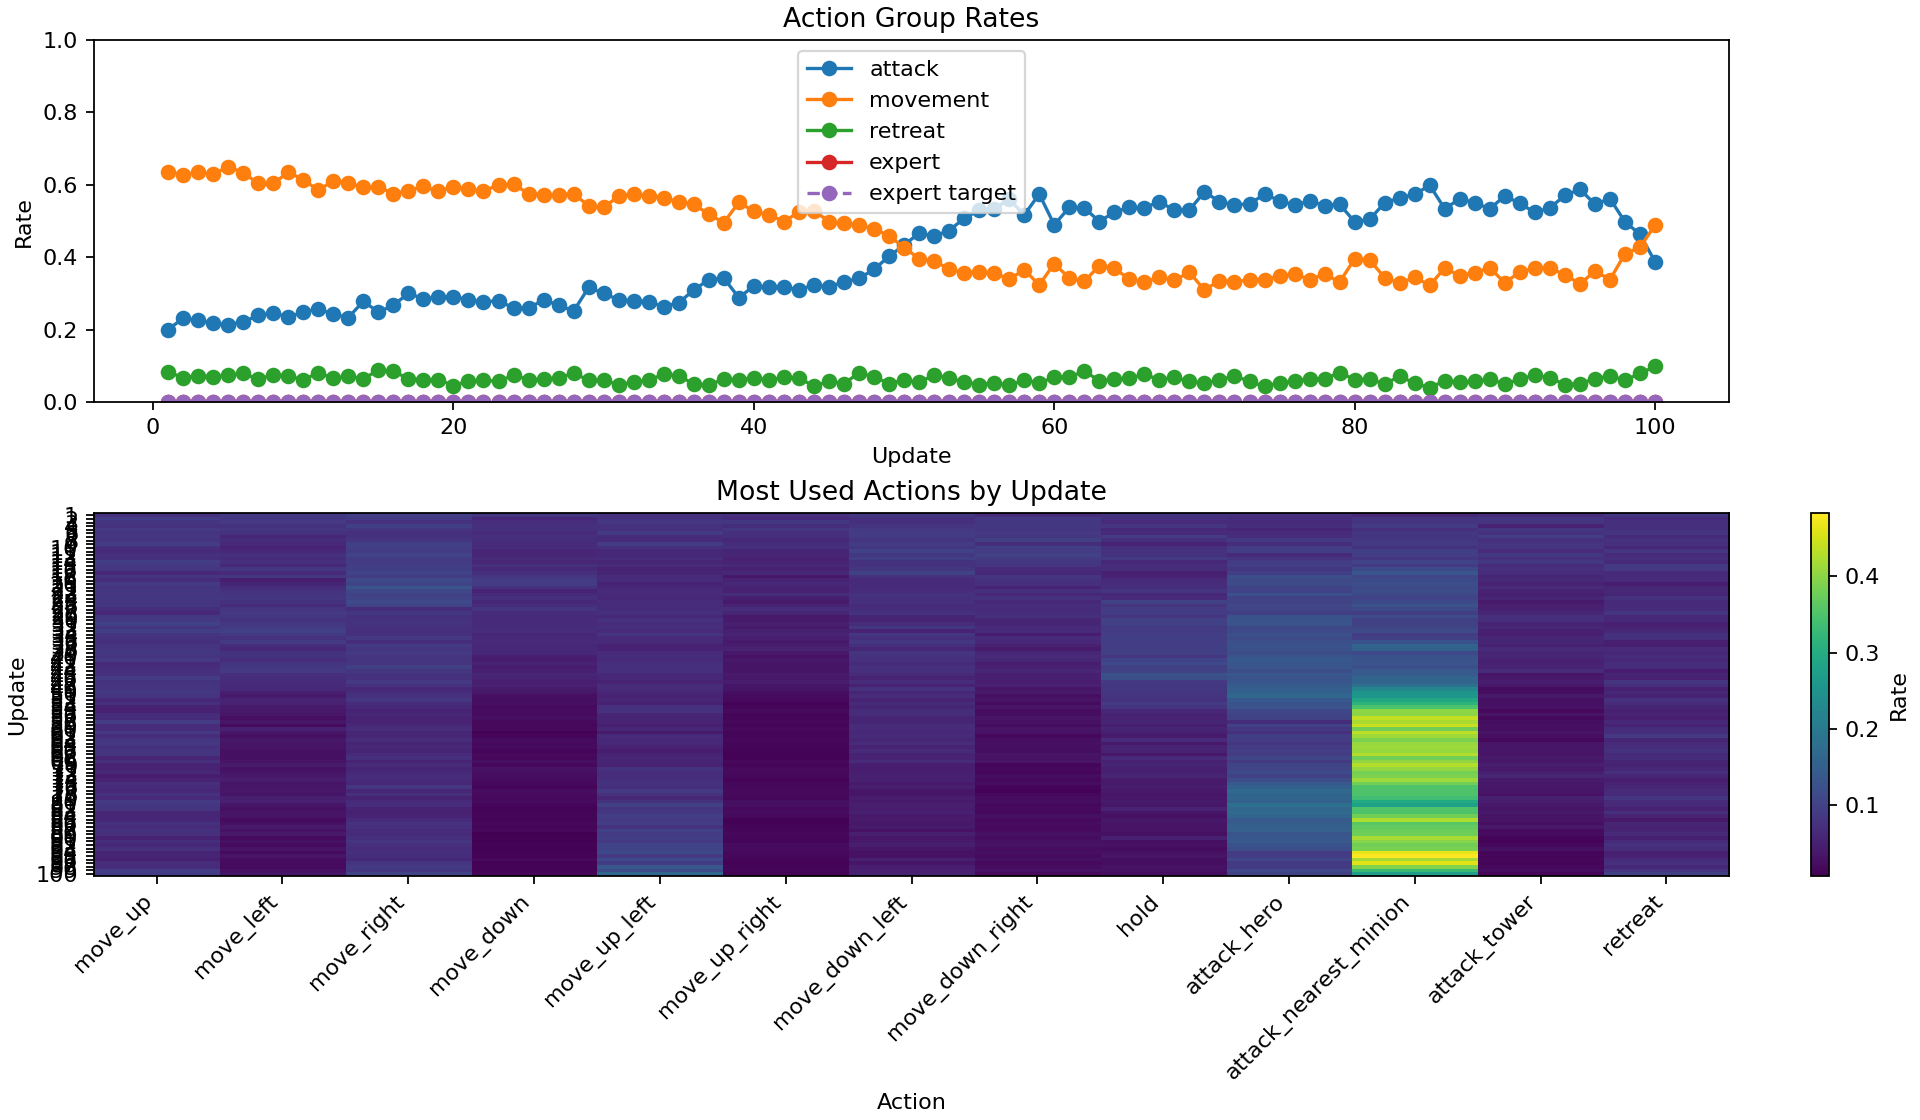
\includegraphics[width=\linewidth]{images/ppo_action_diagnostics.png}
        \caption{Action distribution}
        \label{fig:ppo_action}
    \end{subfigure}
    \hfill
    \begin{subfigure}{0.48\linewidth}
        \centering
        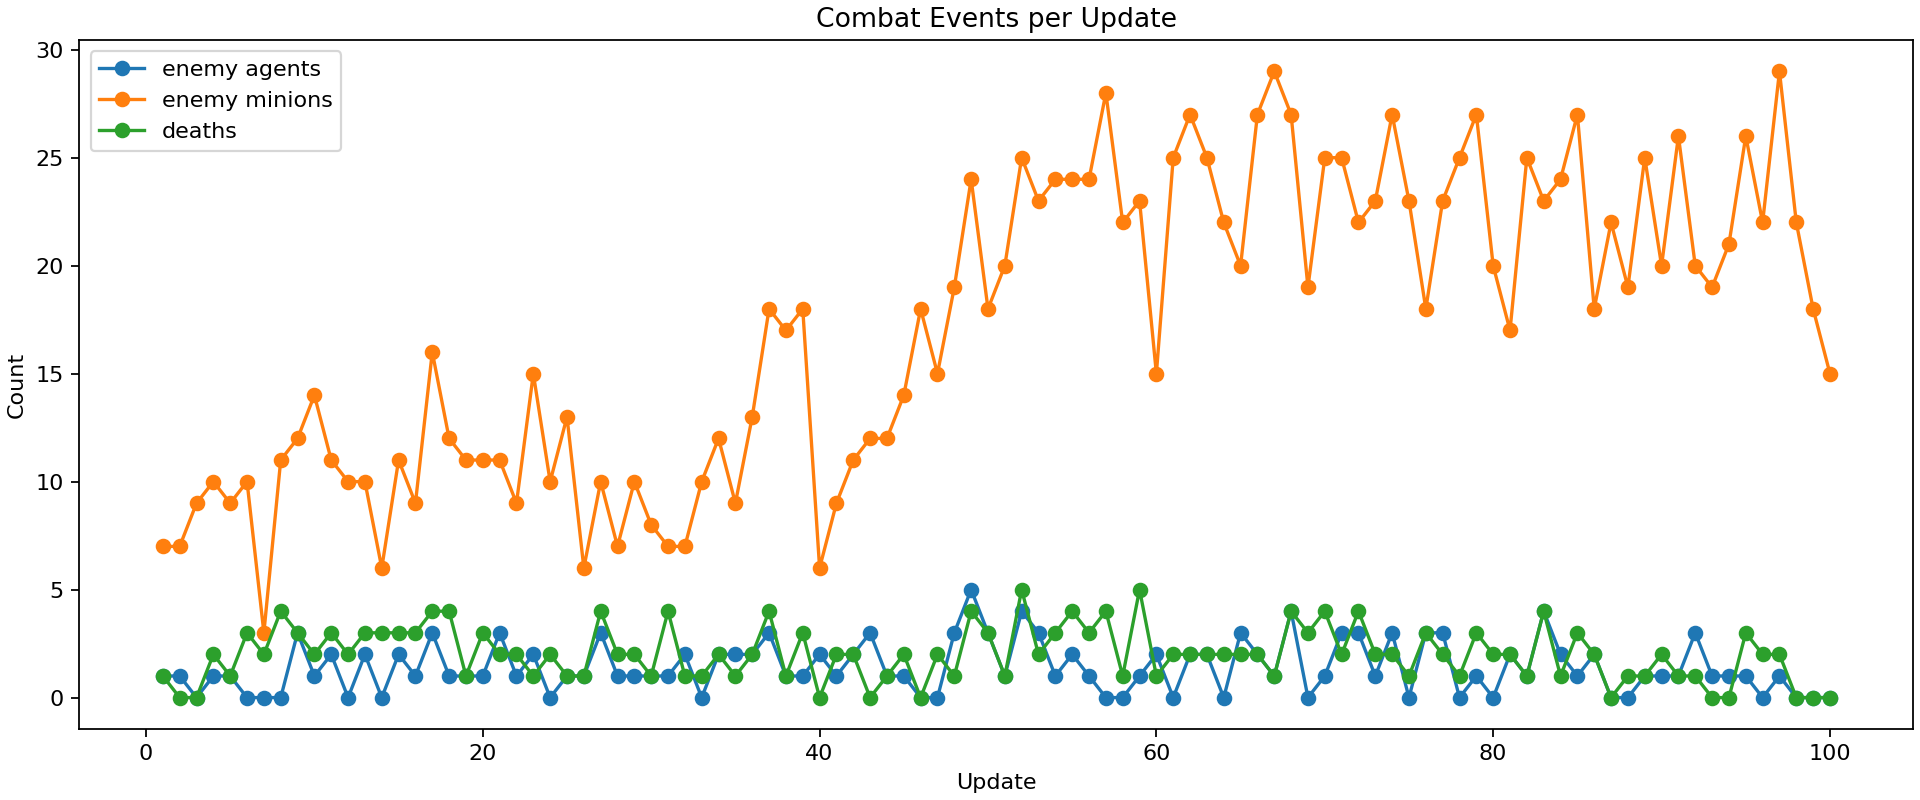
\includegraphics[width=\linewidth]{images/ppo_combat_events.png}
        \caption{Combat events}
        \label{fig:ppo_combat}
    \end{subfigure}

    \vspace{0.5em}

    \begin{subfigure}{0.48\linewidth}
        \centering
        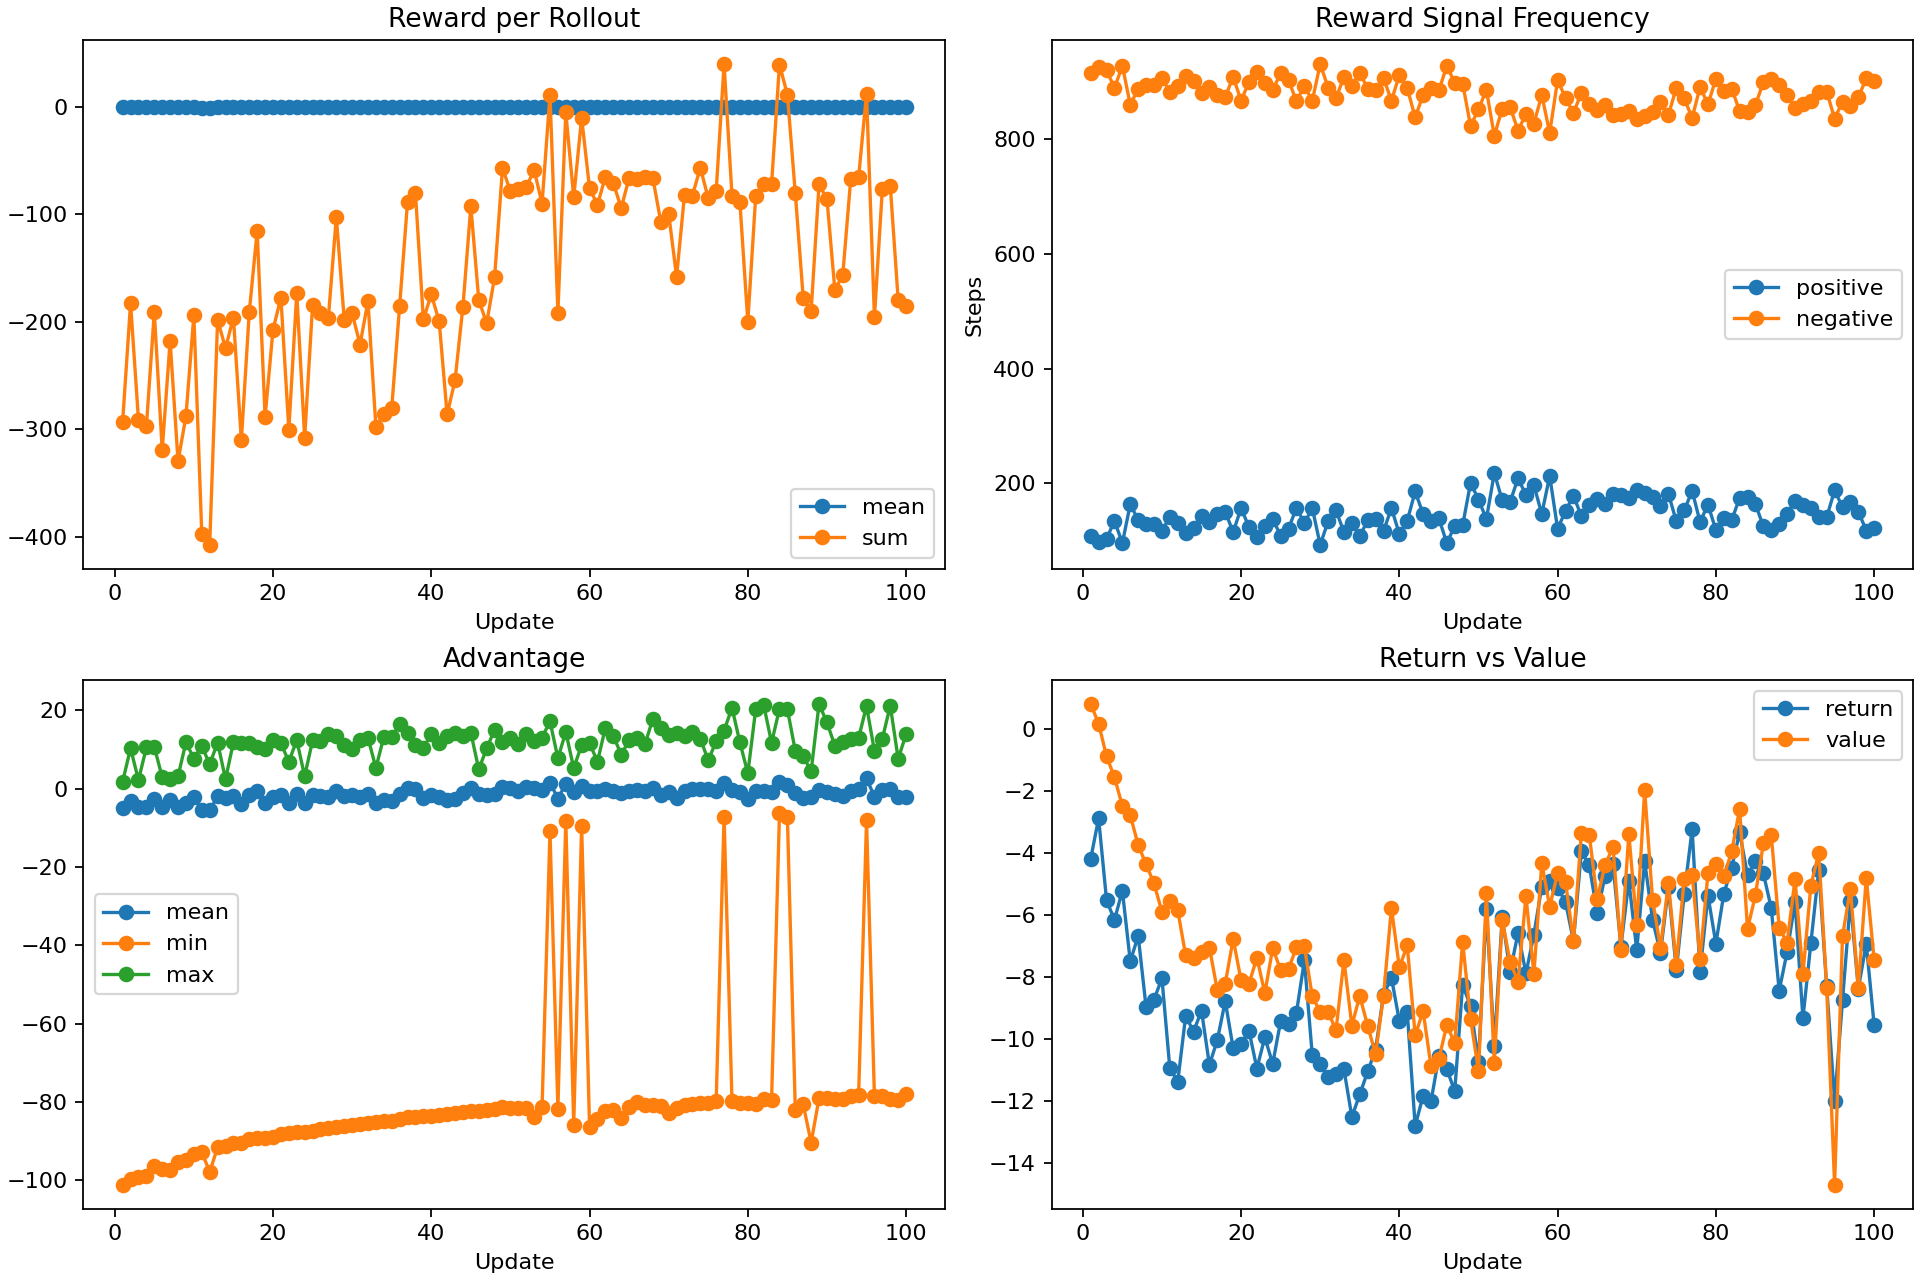
\includegraphics[width=\linewidth]{images/ppo_reward_diagnostics.png}
        \caption{Reward diagnostics}
        \label{fig:ppo_reward}
    \end{subfigure}
    \hfill
    \begin{subfigure}{0.48\linewidth}
        \centering
        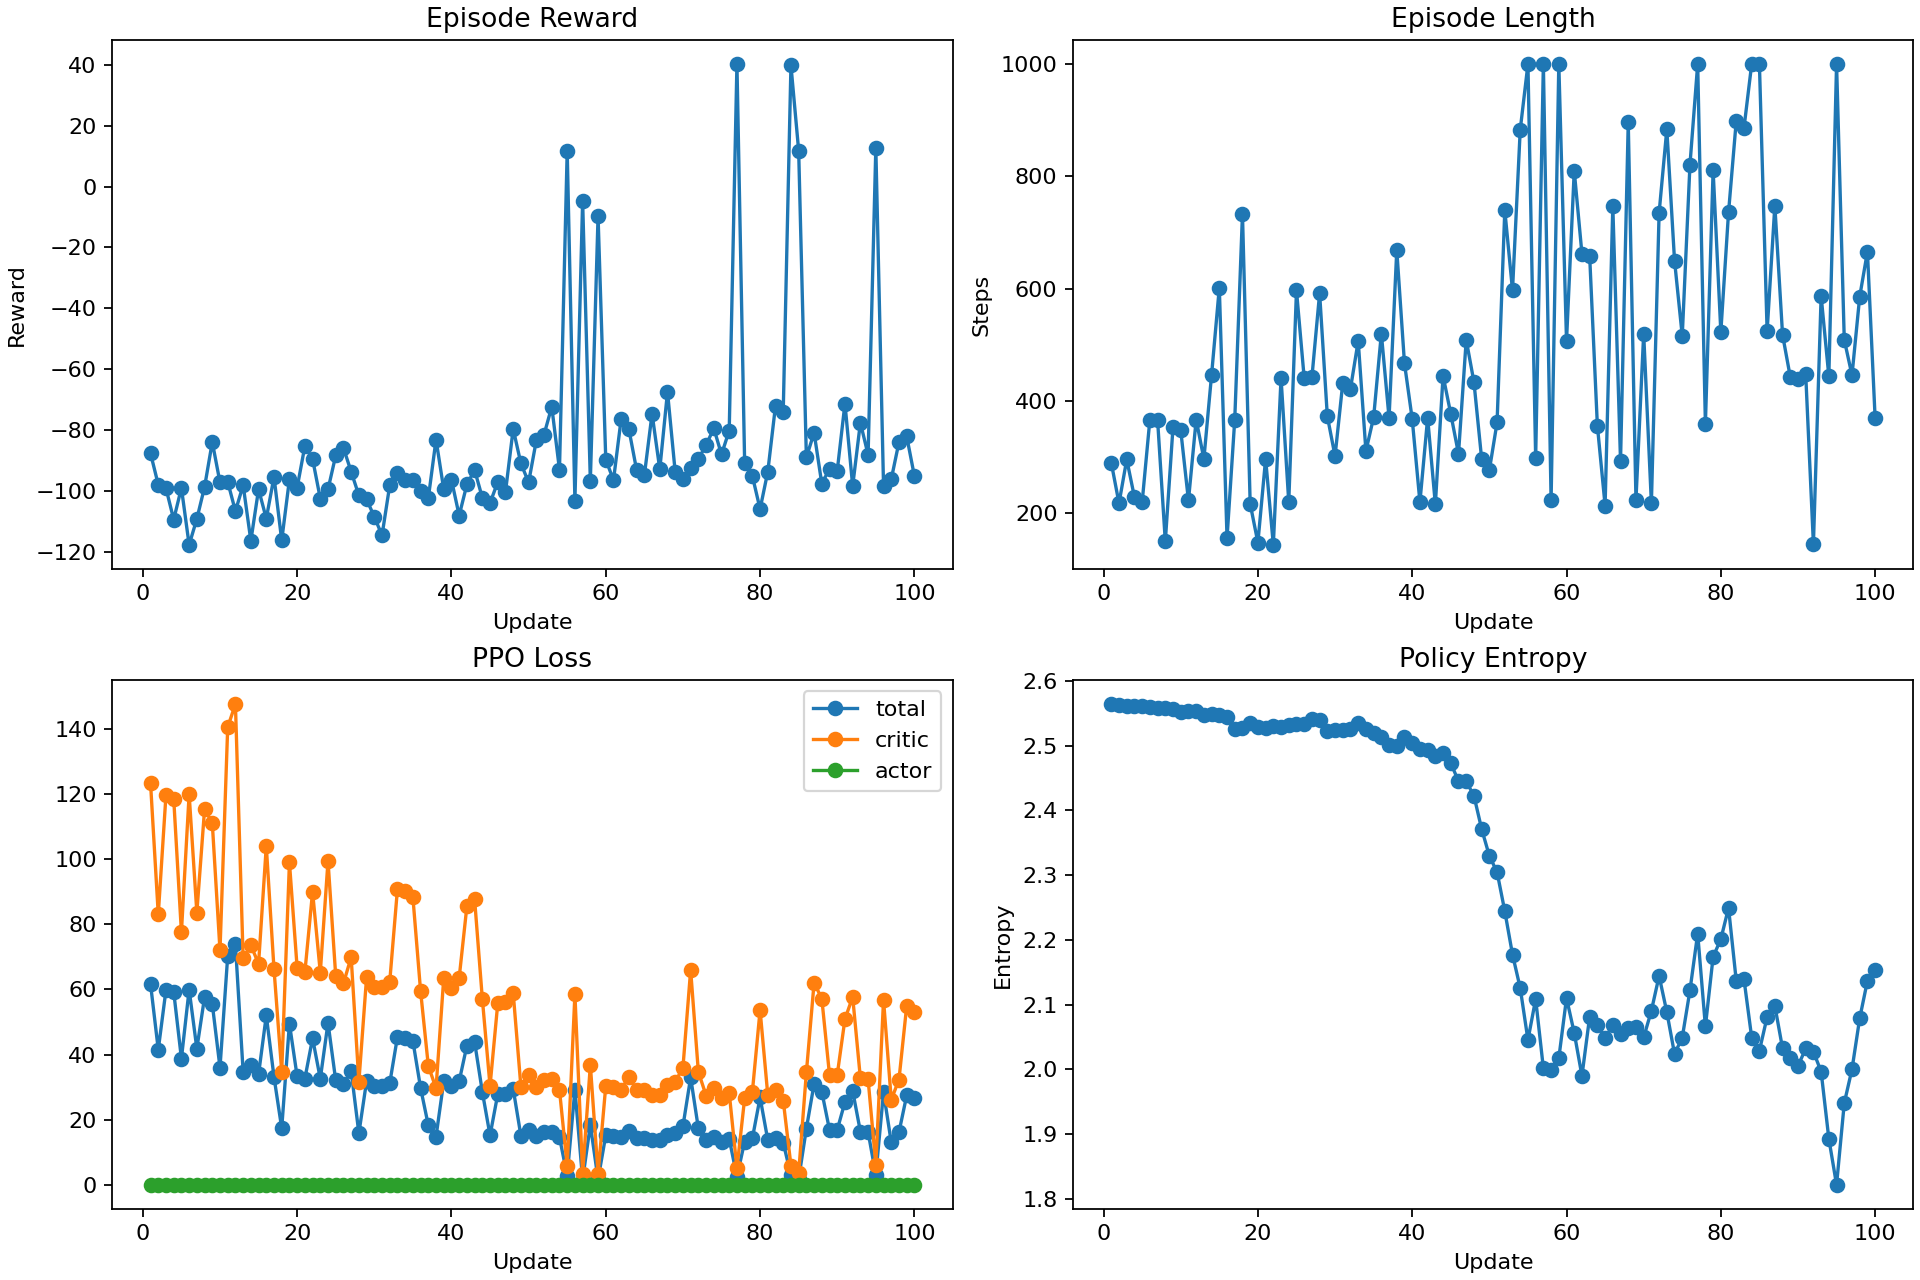
\includegraphics[width=\linewidth]{images/ppo_training_curves.png}
        \caption{Training curves}
        \label{fig:ppo_training}
    \end{subfigure}

    \caption{PPO training diagnostics. The agent gradually shifts toward more attack behavior and learns basic lane-clearing behavior, but reward remains unstable despite decreasing loss and entropy.}
    \label{fig:ppo_diagnostics}
\end{figure}

\subsection{Baseline Selection}

To evaluate the impact of belief-based reasoning, we first establish a strong observation-only baseline.

We compare multiple expert-guided PPO configurations, where expert actions are injected during training with a decaying probability. These configurations differ in the expert policy used for guidance (e.g., aggressive, neutral, farming) as well as the opponent setting during training.

Table~\ref{tab:expert_ranking} summarizes the performance of different configurations. 
Overall, expert-guided PPO significantly outperforms standard PPO, which fails to achieve positive reward across all opponent types. 
Among the expert-guided methods, configurations using aggressive expert guidance consistently achieve higher scores and final rewards.

\begin{table}[h]
\centering
\begin{tabular}{lcc}
\hline
Configuration & Score & Final Reward \\
\hline
aggressiveExpert\_farming & 343.2 & 117.9 \\
aggressiveExpert\_neutral & 268.9 & 82.8 \\
farmingExpert\_neutral & 237.5 & 67.8 \\
neutralExpert\_neutral & 224.8 & 63.2 \\
ppo\_neutral & -65.8 & -71.0 \\
\hline
\end{tabular}
\caption{Comparison of expert-guided PPO configurations.}
\label{tab:expert_ranking}
\end{table}

Although aggressiveExpert\_farming achieves the highest reward, it is specialized to a single opponent type. 
In contrast, aggressiveExpert\_neutral provides a more balanced training signal and better generalization across different opponent behaviors. 
We therefore select aggressiveExpert\_neutral as the baseline for subsequent experiments.

To better understand the effect of expert guidance, we visualize the training dynamics of the selected configuration.

As shown in Figure~\ref{fig:expert_training}, expert-guided PPO achieves substantial improvement in episode reward over training. 
In addition, the action distribution gradually shifts toward more attack-oriented behavior, indicating that the agent learns structured and task-relevant policies under expert guidance.

\begin{figure}[htbp]
\centering


\begin{subfigure}{0.48\linewidth}
    \centering
    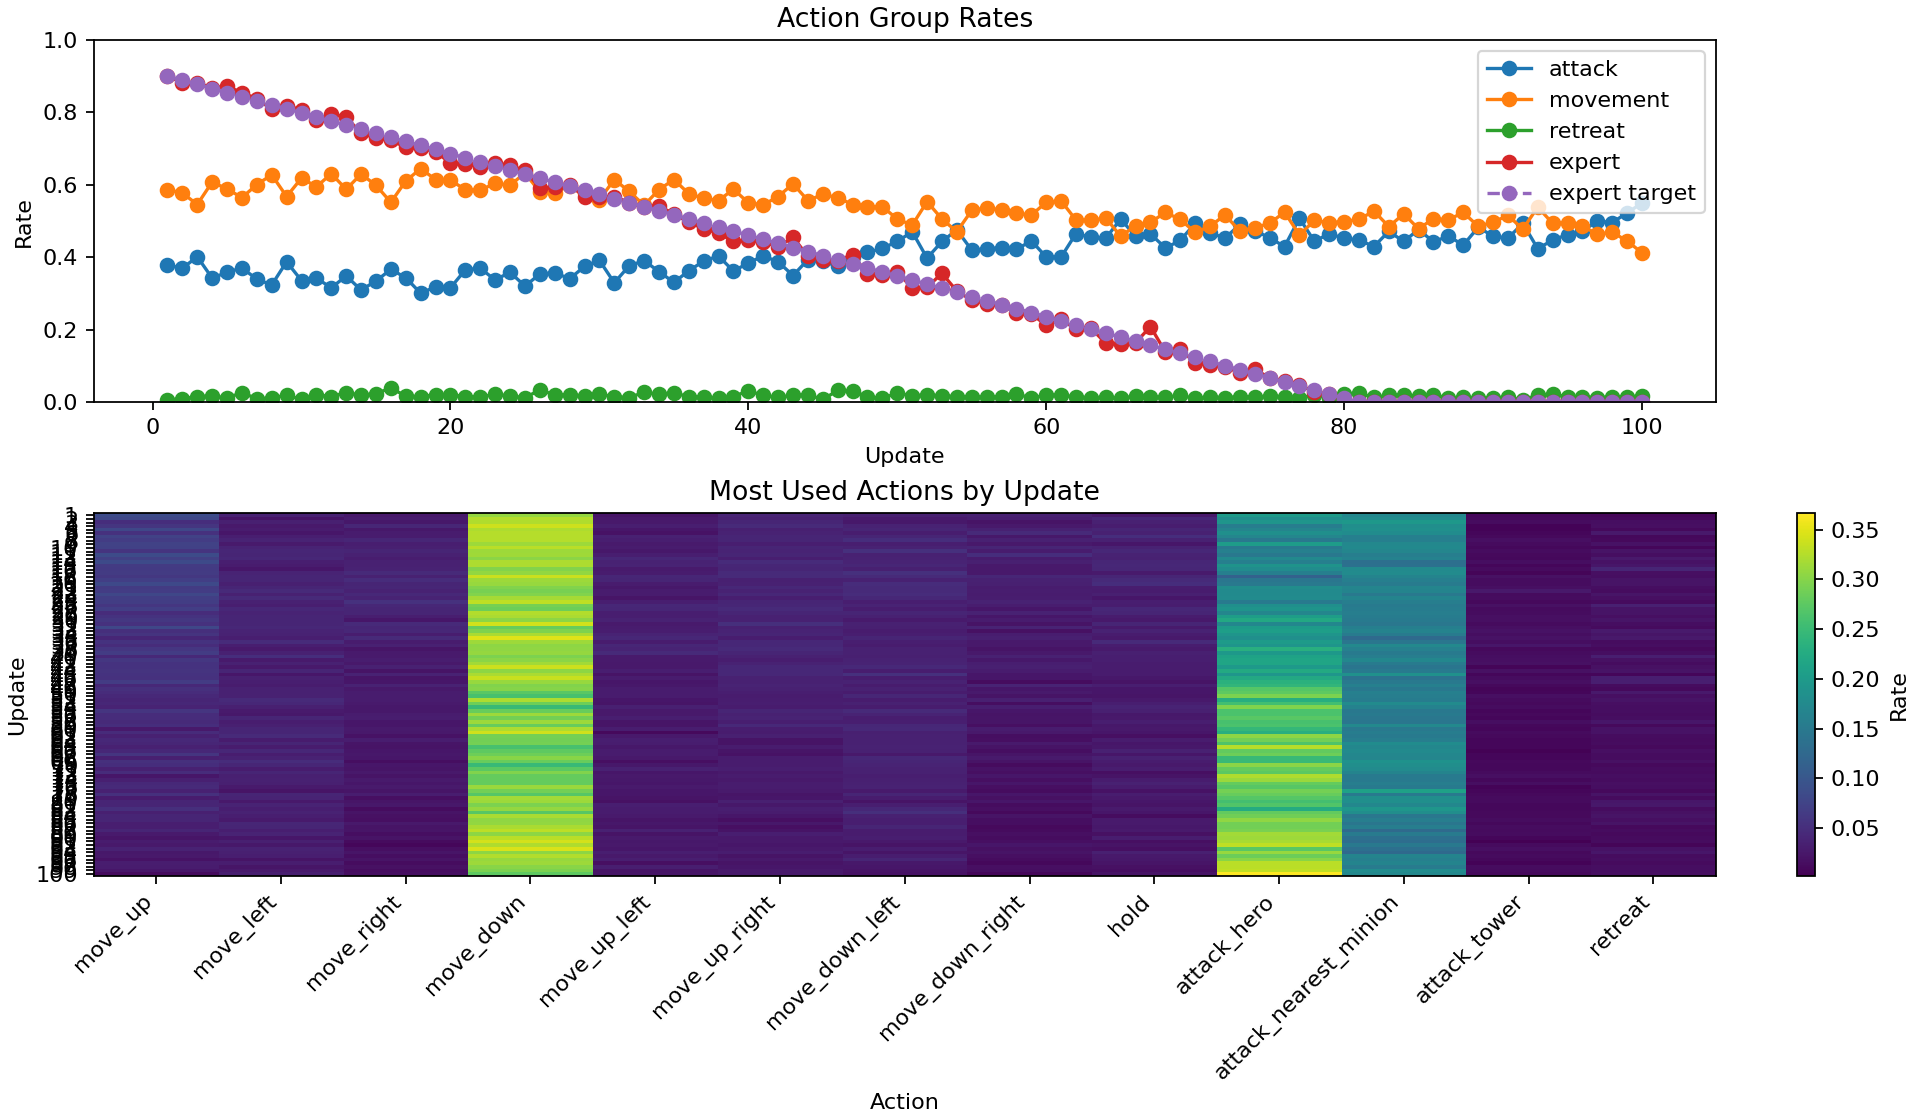
\includegraphics[width=\linewidth]{images/expert_action.png}
    \caption{Action distribution}
\end{subfigure}
\hfill
\begin{subfigure}{0.48\linewidth}
    \centering
    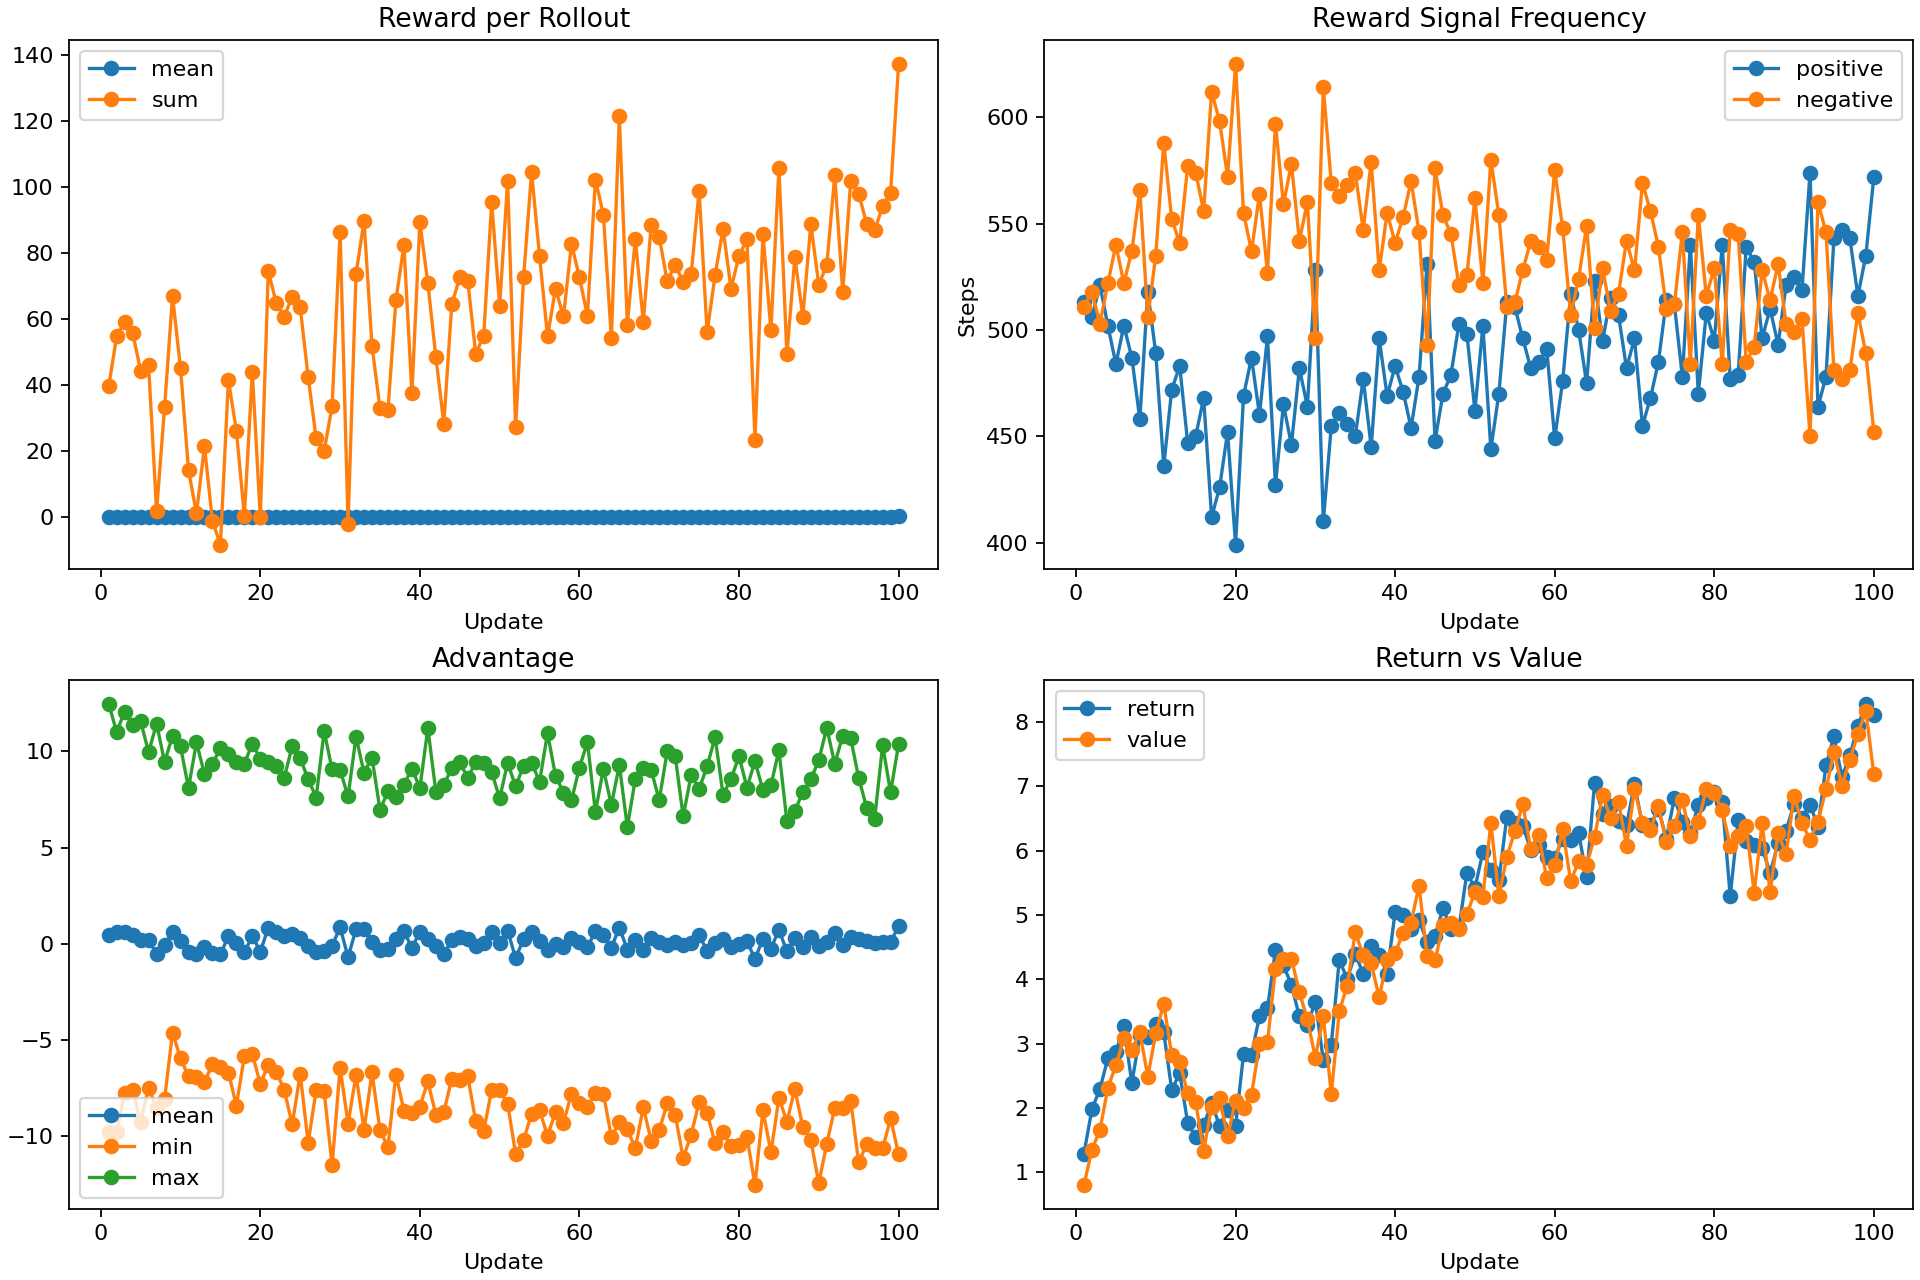
\includegraphics[width=\linewidth]{images/expert_reward.png}
    \caption{Episode reward}
\end{subfigure}

\caption{Training dynamics of expert-guided PPO. The agent achieves higher reward and develops more structured behavior compared to standard PPO.}
\label{fig:expert_training}
\end{figure}

\subsection{Belief Correctness}

Before evaluating whether belief improves policy performance, we first test whether the belief module can infer the opponent's hidden strategy from observations.

At each timestep, we predict the opponent strategy using the maximum-probability belief:
\[
\hat{\theta}_t = \arg\max_{\theta} b_t(\theta).
\]
We then compare this prediction with the ground-truth scripted strategy.

\begin{table}[h]
\centering
\begin{tabular}{lc}
\hline
Strategy & Accuracy \\
\hline
aggressive & 0.8419 \\
neutral & 0.2645 \\
farming & 0.5096 \\
\hline
\end{tabular}
\caption{Belief inference accuracy for fixed opponent strategies.}
\label{tab:belief_accuracy}
\end{table}

As shown in Table~\ref{tab:belief_accuracy}, the belief model identifies aggressive behavior reliably, but performs worse on neutral and farming strategies. 
Neutral is difficult to classify because its behavior overlaps with both aggressive and farming patterns under partial observability.

These results suggest that the belief module provides a meaningful but noisy opponent-strategy signal. 
Therefore, the following experiments should be interpreted as evaluating whether an imperfect belief representation can still improve downstream policy performance.


\subsection{Downstream Policy Performance}

We now evaluate whether incorporating belief improves downstream decision-making.

We compare two policies: an observation-only baseline trained with expert-guided PPO, and a belief-conditioned policy that additionally takes the belief distribution $b_t(\theta)$ as input.

\paragraph{Main Results}

Figure~\ref{fig:downstream} compares observation-only and belief-conditioned policies.

Under fixed opponents, belief-conditioned policies do not achieve higher reward, and in some cases perform slightly worse. 
This suggests that simply providing belief as an additional input is insufficient for improving decision-making. 
Even when belief contains structured information about opponent strategy, the policy may fail to utilize this information effectively.

One possible explanation is that the observation-only policy already captures sufficient behavioral patterns through direct interaction, 
making the additional belief signal redundant. 
Alternatively, the policy network may not learn to associate variations in belief with meaningful changes in action, 
especially when the belief signal is noisy, as observed in Section~5.3.

However, under strategy-switching opponents, belief-conditioned policies exhibit improved stability. 
In particular, action distribution shifts are reduced and reward volatility decreases, 
indicating that belief provides a weak but consistent signal for adapting to non-stationary behavior. 
This suggests that belief may be more useful for stabilizing adaptation rather than improving raw performance.

\paragraph{Belief Ablation}

To further evaluate whether the policy utilizes belief, we conduct ablation experiments by replacing belief with randomized, shuffled, or lagged variants.

As shown in Figure~\ref{fig:ablation}, performance remains largely unchanged across these conditions. 
This indicates that the policy does not strongly depend on belief correctness. 
Even when the belief signal is degraded or randomized, the policy behavior remains largely unchanged.

This suggests that the policy has not learned to rely on belief as a primary decision-making signal, 
but instead continues to depend primarily on direct observations.

\paragraph{Summary}

Taken together, these results highlight a gap between inference and control: 
although the belief module captures structured information about opponent behavior, 
this information is not effectively exploited by the policy to improve reward.

This suggests that explicit belief modeling alone is insufficient. 
Future work should focus on tighter integration between belief inference and policy learning, 
such as end-to-end training or architectures that more directly couple belief dynamics with action selection.

\begin{figure}[htbp]
\centering

\begin{subfigure}{0.48\linewidth}
    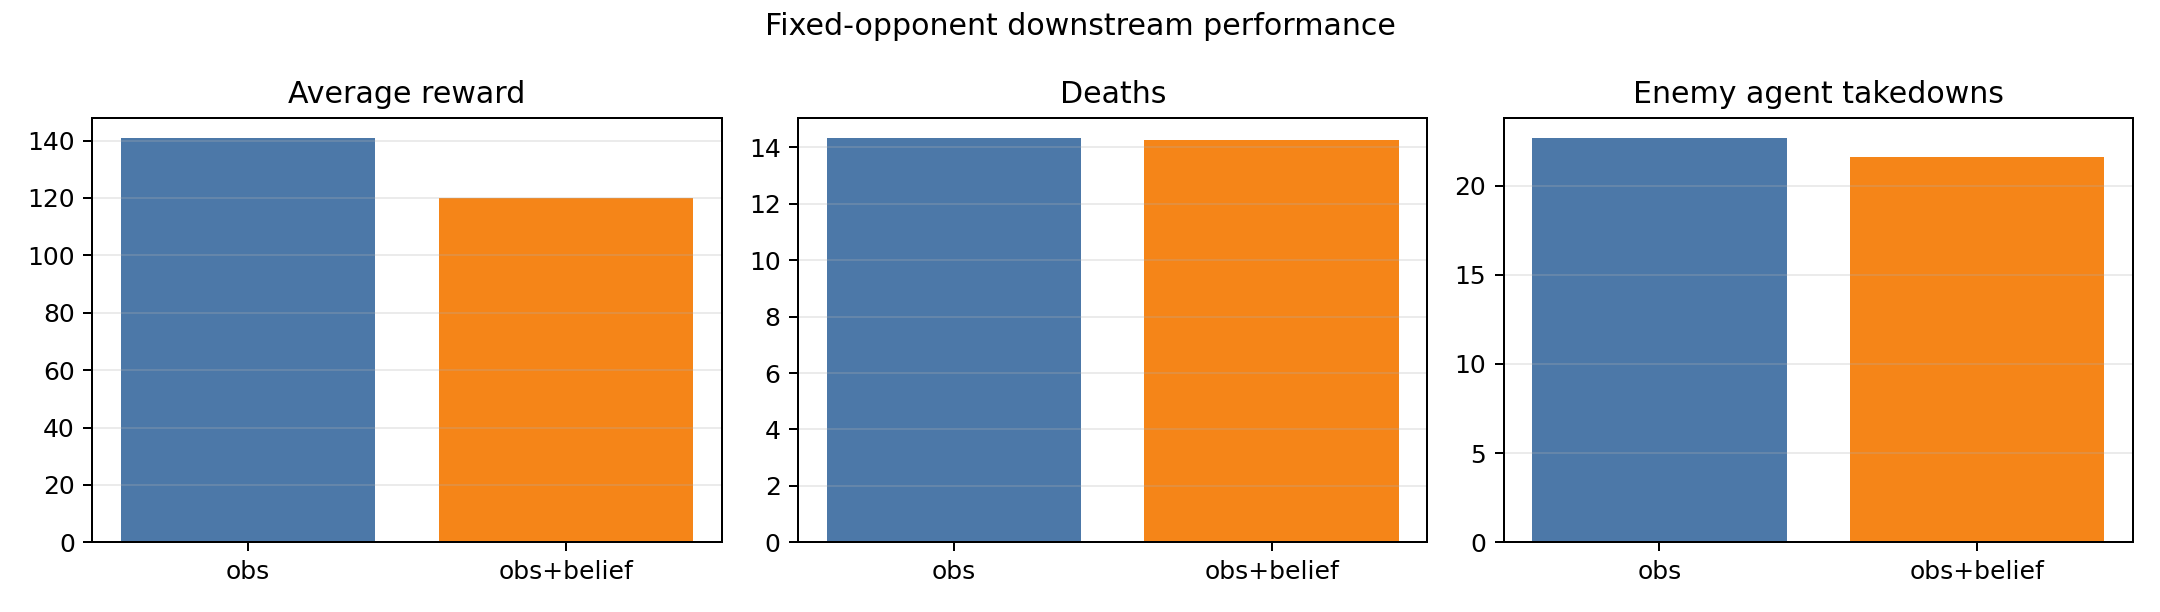
\includegraphics[width=\linewidth]{images/downstream_fixed.png}
    \caption{Fixed-opponent performance}
\end{subfigure}
\hfill
\begin{subfigure}{0.48\linewidth}
    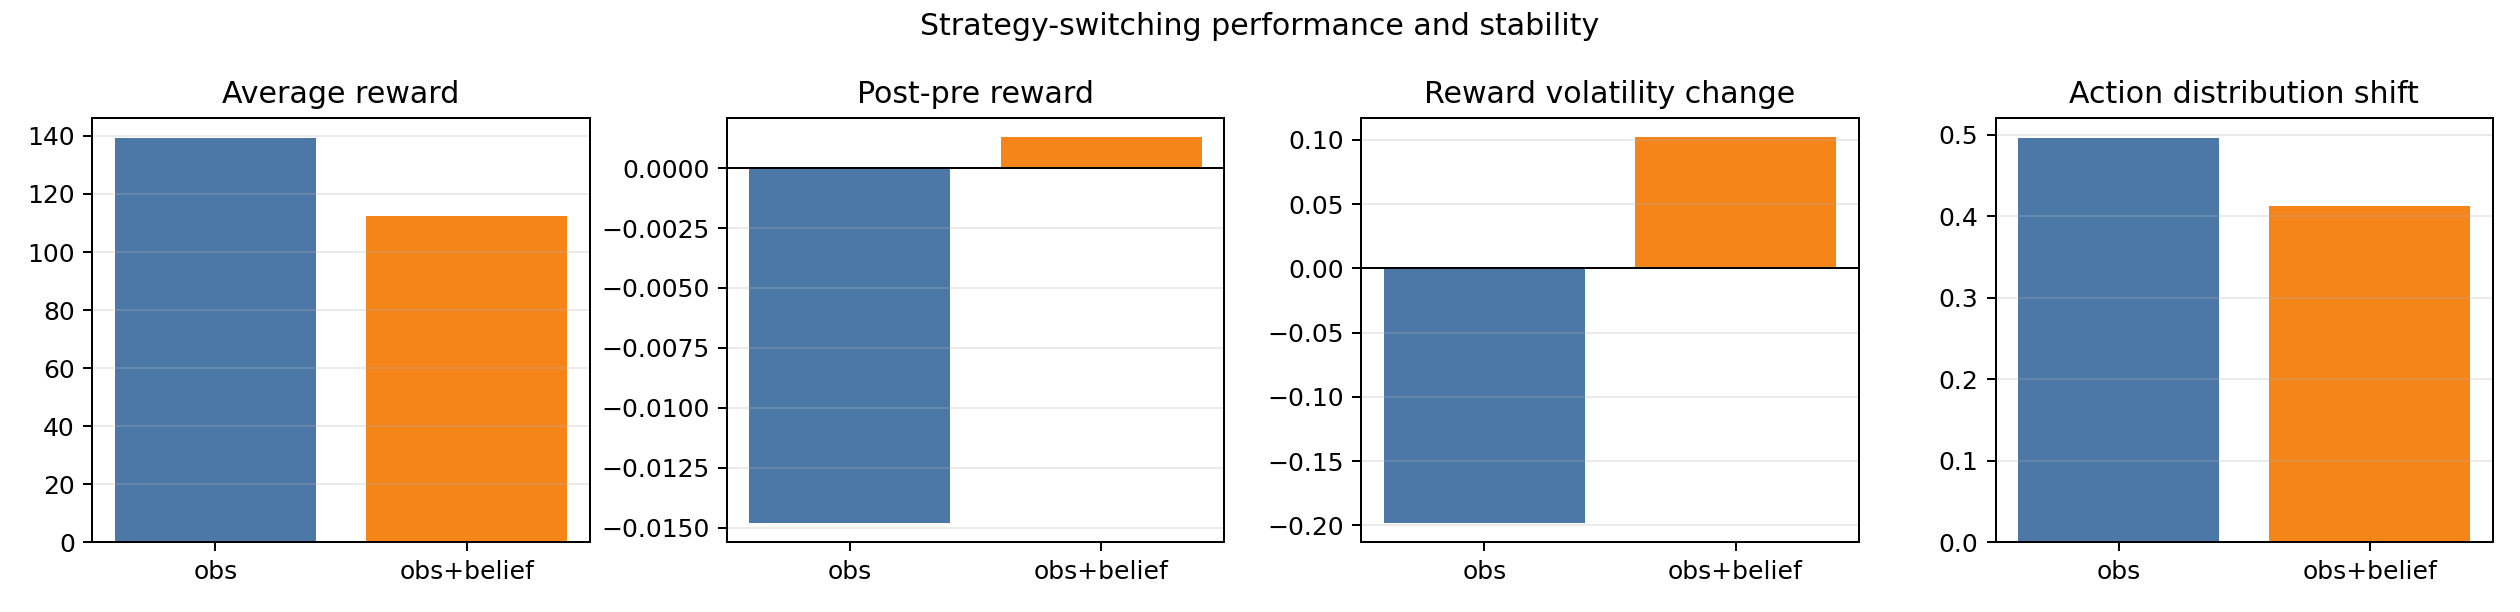
\includegraphics[width=\linewidth]{images/switching_stability.png}
    \caption{Strategy-switching performance}
\end{subfigure}

\caption{Downstream policy performance. 
Belief-conditioned policies do not improve reward under fixed opponents, 
but provide modest improvements in behavioral stability under strategy switching.}
\label{fig:downstream}
\end{figure}

\begin{figure}[htbp]
\centering
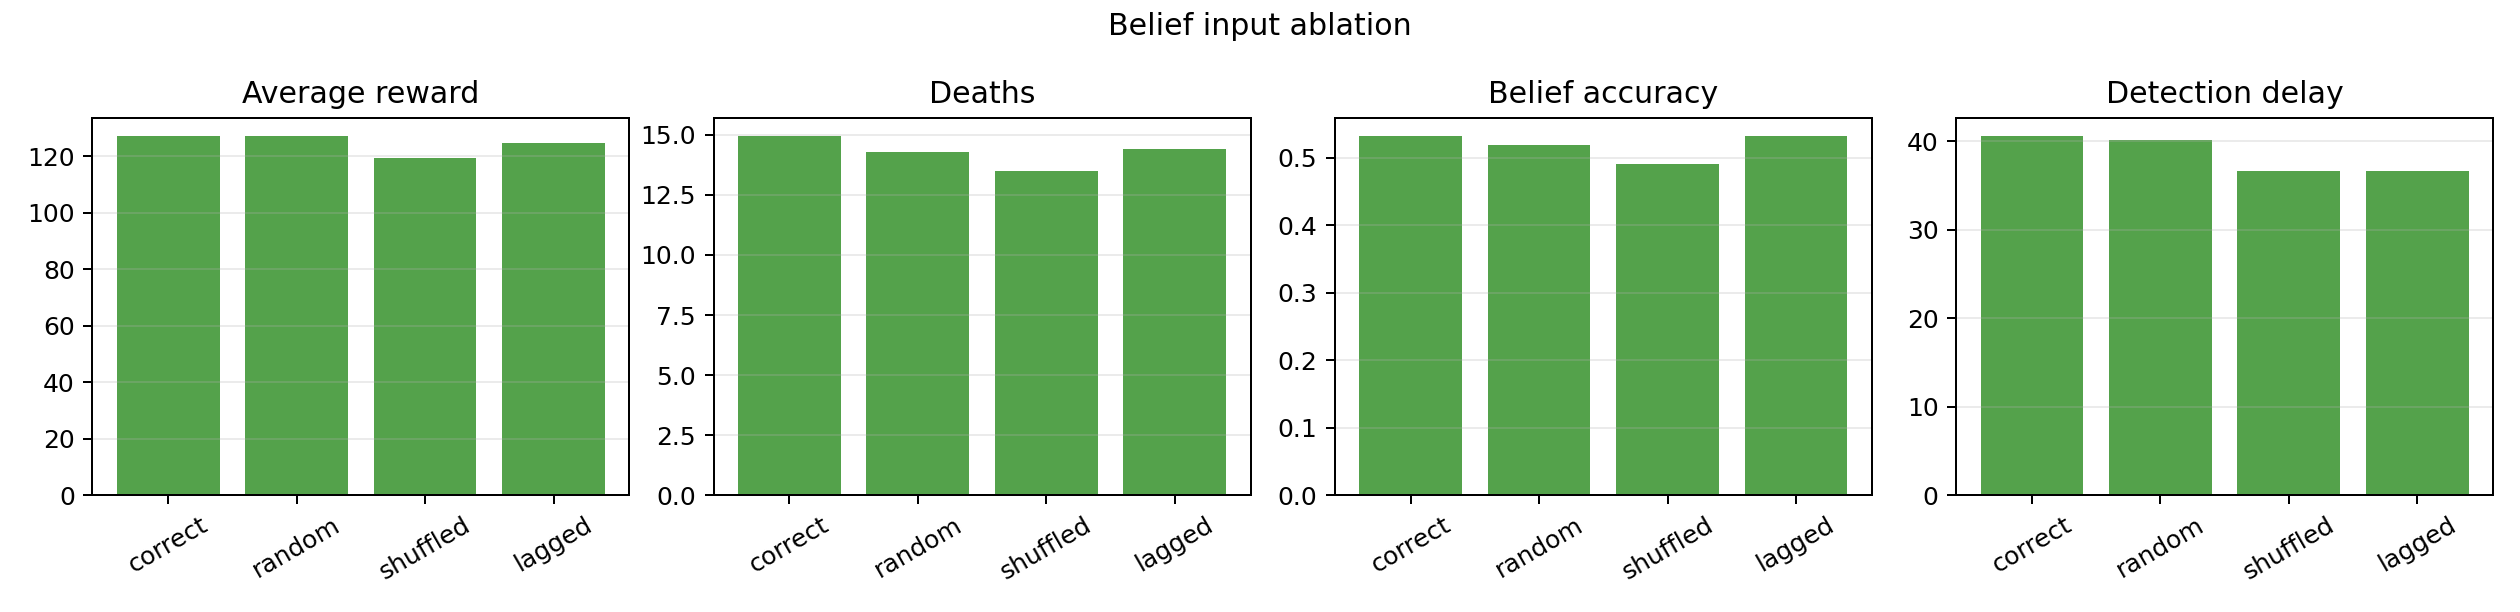
\includegraphics[width=0.9\linewidth]{images/belief_ablation.png}
\caption{Belief input ablation. Replacing belief with random or shuffled signals does not significantly affect performance, 
indicating that the policy does not strongly depend on belief correctness.}
\label{fig:ablation}
\end{figure}

\section{Discussion}

Our results provide several insights into the role of belief-based reasoning in partially observable, non-stationary environments.

\paragraph{Imperfect Belief as a Limitation}

First, the belief model itself is imperfect, particularly for neutral strategies. 
As shown in Section~5.3, neutral behavior is difficult to distinguish because it overlaps with both aggressive and farming patterns under partial observability. 
This ambiguity limits the quality of the belief signal and may reduce its usefulness for downstream decision-making.

\paragraph{Policy Does Not Utilize Belief}

More importantly, our ablation results suggest that the policy does not effectively utilize belief information. 
Even when the belief signal is randomized or degraded, policy performance remains largely unchanged. 
This indicates that the learned policy relies primarily on direct observations rather than explicitly inferred opponent strategies.

\paragraph{Observation May Be Sufficient}

One possible explanation is that the observation space already contains sufficient information for decision-making. 
Through interaction, the policy may implicitly capture behavioral patterns without requiring an explicit belief representation. 
In such cases, belief becomes redundant unless it provides information that is otherwise inaccessible.

\paragraph{Belief Helps Stability but Not Performance}

Despite not improving reward, belief-conditioned policies exhibit improved stability under strategy switching. 
This suggests that belief may serve as a regularizing signal that smooths policy responses to non-stationary behavior, 
rather than directly improving task performance.

\paragraph{Implications for RL and Multi-Agent Systems}

These findings highlight a gap between inference and control: 
even when structured information about the environment is available, 
it is not automatically exploited by the policy. 
This suggests that explicit reasoning modules must be more tightly integrated with policy learning in order to be effective.

\paragraph{Limitations}

This work has several limitations. 
The belief model relies on heuristic scoring functions rather than learned representations, 
which may restrict its expressiveness. 
In addition, the environment is simplified and focuses on a limited set of strategies. 
Finally, the policy architecture is relatively simple and may not be sufficient to fully leverage belief inputs.

\paragraph{Future Work}

Future work should explore end-to-end learning of belief representations, 
as well as architectures that more explicitly couple belief inference with policy updates. Another natural extension is power scaling through experience gain: minion and neutral-monster takedowns could grant XP that increases agent strength over time, creating a clearer strategic incentive to farm lane and jungle resources instead of only pursuing immediate combat outcomes. 
Extending the framework to more complex multi-agent settings, including cooperative scenarios, richer progression systems, and unseen strategies, 
would further test the usefulness of belief-based reasoning.

\section{Conclusion}

In this work, we studied belief-based opponent modeling in a partially observable, non-stationary environment.

We showed that belief inference can capture meaningful information about opponent strategies, 
particularly for clearly distinguishable behaviors such as aggressive play. 
However, belief accuracy remains limited in ambiguous cases such as neutral strategies.

More importantly, we found that incorporating belief into the policy does not improve downstream reward. 
Through ablation experiments, we observed that the policy does not strongly depend on belief correctness, 
suggesting that the inferred information is not effectively utilized.

Despite this, belief-conditioned policies exhibit improved stability under strategy switching, 
indicating that belief provides a weak but consistent signal for handling non-stationarity.

Overall, our results suggest that while belief modeling provides interpretable structure, 
it is not sufficient on its own to improve decision-making. 
Bridging the gap between inference and control remains an important direction for future research in reinforcement learning and multi-agent systems.

\FloatBarrier

\newpage
\bibliographystyle{plainnat}
\bibliography{references}

\end{document}
